\documentclass[11pt,a4paper]{article}

\usepackage{fontspec}
\usepackage{polyglossia}
\setmainlanguage{portuguese}
\usepackage{amsmath,amssymb,amsthm}
\usepackage{booktabs}
\usepackage{graphicx}
\usepackage{listings}
\usepackage{xcolor}
\usepackage{enumitem}
\usepackage[a4paper,margin=2.5cm]{geometry}
\usepackage[hidelinks]{hyperref}

\emergencystretch=3em
\setlength{\parskip}{0.5em}
\setlength{\parindent}{0pt}

\newcommand{\repourl}{\href{https://github.com/SEU-USUARIO/lab-bolsistas-capes}{\nolinkurl{https://github.com/SEU-USUARIO/lab-bolsistas-capes}}}
      % define \repourl (gerado por "make relatorio")
\newcommand{\totalpontos}{10}
\newcommand{\maiorN}{5.120}
\newcommand{\inclinacao}{1,988}
\newcommand{\cnnMaior}{0,5001}
\newcommand{\razaoMaior}{3,999}
\newcommand{\cLidas}{6.250}
\newcommand{\cInseridos}{6.000}
\newcommand{\cRedundantes}{250}
\newcommand{\cComp}{18.761.097}
\newcommand{\cBase}{18.003.000}
\newcommand{\cExcesso}{758.097}
\newcommand{\cMedia}{3032,4}
\newcommand{\ambCompilador}{gcc (Ubuntu 13.3.0-6ubuntu2\textasciitilde{}24.04.1) 13.3.0}
\newcommand{\ambSistema}{Linux 6.18.44-fc-v139}
\newcommand{\ambData}{15/10/2026}
 % macros com os valores medidos

\newtheorem{teorema}{Teorema}
\newtheorem{lema}{Lema}

\lstset{
  language=C, basicstyle=\ttfamily\footnotesize, numbers=left,
  numberstyle=\tiny\color{gray}, frame=single, breaklines=true,
  keywordstyle=\bfseries, commentstyle=\color{gray!70!black},
  columns=fullflexible, keepspaces=true, showstringspaces=false
}

\title{Análise de Algoritmos Aplicada ao Cadastro de Bolsistas da CAPES\\[0.4em]
       \large Relatório 3 --- Laboratório 10/09}
\author{Wilton Rodrigues do Carmo Filho\\
        Grupo 17\\
        Análise de Algoritmos (GPE02M60042) --- Universidade Católica de Brasília}
\date{15 de outubro de 2026}

\begin{document}
\renewcommand{\proofname}{Demonstração}
\maketitle

\noindent\fbox{\parbox{\dimexpr\linewidth-2\fboxsep-2\fboxrule\relax}{%
\textbf{Repositório Git público:} \repourl\\
Contém o código-fonte em C, o arquivo \texttt{bolsistas-2025.csv}, os arquivos de
entrada dos testes, os CSV gerados nos experimentos, as saídas do programa,
os scripts, as instruções de compilação e de execução (\texttt{README.md}) e a
fonte deste relatório.}}

\tableofcontents

%--------------------------------------------------------------------------
\section{Introdução}

A CAPES recebe solicitações de cadastro de bolsistas em arquivos CSV que precisam
ser incorporadas ao cadastro principal sem gerar registros duplicados. Este
trabalho implementa em C um programa, chamado \texttt{copiador}, que copia os
registros de um CSV de origem para um CSV de destino ignorando qualquer registro
cujo campo \emph{Nome} já exista no destino, e que conta o número de comparações
entre nomes realizadas pela busca de redundância.

O objetivo central, porém, é a análise do algoritmo. O relatório (i) deduz uma
função $C(n)$ para o número de comparações necessárias para inserir $n$ nomes
distintos, (ii) demonstra por indução matemática que a expressão deduzida
está correta, (iii) classifica o algoritmo assintoticamente, (iv) mede $C(n)$
experimentalmente com o contador implementado e (v) confronta as previsões
teóricas com as medições.

%--------------------------------------------------------------------------
\section{Descrição da solução implementada}

O programa recebe, pela linha de comando, o CSV de origem, o CSV de destino e o
CSV de estatísticas:

\begin{center}\texttt{./copiador bolsistas-2025.csv cadastro.csv estatisticas.csv}\end{center}

As regras implementadas seguem o enunciado:
\begin{itemize}[nosep]
  \item \textbf{Critério de redundância:} somente o campo \emph{Nome} (primeiro
        campo) é comparado, por igualdade exata de texto (\texttt{strcmp}, sem
        normalização de caixa ou de espaços). Duas linhas com o mesmo Nome e
        demais campos diferentes são redundantes.
  \item \textbf{Cópia:} um registro não redundante é copiado \emph{inteiro}
        (todos os campos originais) para o final do destino.
  \item \textbf{Redundância:} para um registro redundante o programa escreve na
        saída padrão \texttt{ERRO: nome redundante encontrado: <nome>},
        não o copia e continua o processamento.
  \item \textbf{Cabeçalhos:} se o destino não existe ou está vazio, o programa cria
        o cabeçalho \texttt{Nome,Modalidade,Nivel,Agencia}. A primeira linha da
        origem, quando é o cabeçalho, não é copiada como registro.
  \item \textbf{Estatísticas:} ao final, uma linha
        \texttt{nomes\_inseridos,comparacoes} é anexada ao arquivo de estatísticas
        (o cabeçalho é escrito se o arquivo é novo).
\end{itemize}

\paragraph{Convenção de contagem.} Cada vez que o Nome de um registro da origem é
comparado com o Nome de uma linha do destino, o contador é incrementado em uma
unidade. A busca é sequencial e percorre \emph{todas as linhas do arquivo de
destino}, e o cabeçalho é uma linha desse arquivo (seu campo Nome vale
\texttt{Nome}). Portanto o cabeçalho participa da busca e conta como uma
comparação. Essa convenção é a que reproduz o exemplo de saída do enunciado
(10 nomes $\rightarrow$ 55 comparações, 20 $\rightarrow$ 210 etc.), como
mostrado na Seção~\ref{sec:analise}.

%--------------------------------------------------------------------------
\section{Explicação do funcionamento do programa}

A execução segue estes passos:
\begin{enumerate}[nosep]
  \item Carrega o arquivo de destino, se existir, para um vetor com o Nome de cada
        linha, na mesma ordem em que aparecem no arquivo. Se o destino não existe
        ou está vazio, escreve o cabeçalho e o registra como primeira linha do vetor.
  \item Abre a origem e lê uma linha por vez. Linhas em branco são ignoradas.
  \item Extrai o Nome (primeiro campo; aceita campo entre aspas).
  \item Executa a busca sequencial do Nome no vetor, incrementando o contador a
        cada comparação.
  \item Se encontrou: imprime a mensagem de erro e segue para a próxima linha.
        Se não encontrou: anexa a linha completa ao destino, acrescenta o Nome ao
        vetor e incrementa \texttt{inseridos}.
  \item Ao final, anexa \texttt{inseridos,comparacoes} ao arquivo de estatísticas.
\end{enumerate}

O núcleo do algoritmo e da instrumentação é a função abaixo (trecho de
\texttt{src/copiador.c}):
\begin{lstlisting}
static unsigned long long comparacoes = 0;

static int nome_existe(const Cadastro *c, const char *nome)
{
    for (size_t i = 0; i < c->tamanho; i++) {
        comparacoes++;                          /* uma comparacao */
        if (strcmp(c->nomes[i], nome) == 0)
            return 1;                           /* redundante */
    }
    return 0;                                   /* nome novo */
}
\end{lstlisting}

\paragraph{Exemplo do enunciado.} Com o destino contendo o cabeçalho e
\texttt{MARIA APARECIDA SILVA,DS,M,CAPES}, e a origem contendo
\texttt{MARIA APARECIDA SILVA,PQ,C,CNPq} e
\texttt{ABILIO AZAMBUJA RODRIGUES FILHO,PQ,C,CNPq}, a saída padrão é
\texttt{ERRO: nome redundante encontrado: MARIA APARECIDA SILVA}, o destino
passa a ter 3 linhas (a de ABILIO é a nova) e as estatísticas registram
\texttt{1,4}: o primeiro nome é achado na 2.ª linha do destino (2 comparações) e
o segundo percorre as 2 linhas sem achar (2 comparações). Esse caso é um dos
testes automatizados (\texttt{make test}).

%--------------------------------------------------------------------------
\section{Estruturas de dados utilizadas}

\begin{itemize}[nosep]
  \item \textbf{\texttt{Cadastro}}: um vetor dinâmico de \texttt{char *} com o
        Nome de cada linha do destino, mais o tamanho e a capacidade. A
        capacidade dobra quando se esgota (\texttt{realloc}), de modo que o
        acréscimo é $O(1)$ amortizado. A posição $i$ do vetor corresponde à
        $i$-ésima linha do arquivo de destino, de modo que percorrer o vetor
        em ordem é exatamente a busca sequencial sobre o arquivo.
  \item \textbf{Contador} \texttt{comparacoes}: variável global do tipo
        \texttt{unsigned long long}, incrementada em cada passo da busca.
  \item \textbf{Buffers de linha}: alocados por \texttt{getline}, sem limite fixo
        de tamanho de linha ou de quantidade de registros.
\end{itemize}

Uma tabela de dispersão (\emph{hash}) reduziria o custo esperado da busca para
$O(1)$, mas mudaria o algoritmo que o exercício pede para analisar (busca
sequencial); por isso foi mantido o vetor. O vetor em memória evita reabrir e
reler o arquivo a cada verificação, sem alterar a contagem de comparações, pois
cada elemento do vetor representa uma linha do destino.

%--------------------------------------------------------------------------
\section{Análise teórica do algoritmo}
\label{sec:analise}

\paragraph{Hipóteses.} (H1) a verificação de redundância é uma busca sequencial;
(H2) os $n$ nomes a inserir são distintos entre si e distintos dos já existentes;
(H3) o destino inicia contendo apenas o cabeçalho.

\paragraph{Custo de uma inserção.} Antes da $k$-ésima inserção ($k=1,\dots,n$) o
destino tem $k$ linhas: o cabeçalho e os $k-1$ registros já inseridos. Pela
hipótese H2 nenhuma delas é igual ao novo nome, então a busca percorre as $k$
linhas e faz exatamente $k$ comparações.

\paragraph{Questão 2: função $C(n)$.} O total é a soma dos custos:
\[
  C(n) \;=\; \sum_{k=1}^{n} k \;=\; \frac{n(n+1)}{2} \;=\; \frac{n^2}{2}+\frac{n}{2}.
\]
A dedução detalhada está na Seção~\ref{sec:deducao} e a demonstração por indução
na Seção~\ref{sec:inducao}.

\paragraph{Questão 1: comparações para cada $n$.}
\begin{center}
\begin{tabular}{rr}
\toprule
$n$ & $C(n)=n(n+1)/2$ \\
\midrule
10  & 55 \\
20  & 210 \\
40  & 820 \\
80  & 3.240 \\
160 & 12.880 \\
\bottomrule
\end{tabular}
\end{center}
Esses valores coincidem com o exemplo de saída do enunciado.

\paragraph{Questão 3: complexidade assintótica.} $C(n)=\frac{n^2}{2}+\frac{n}{2}\le n^2$
para todo $n\ge 1$ (pois $\frac{n+1}{2}\le n$), logo $C(n)\in O(n^2)$ com $c=1$ e
$n_0=1$. Como também $C(n)\ge \frac{n^2}{2}$, vale $C(n)\in\Theta(n^2)$. As
demais operações (leitura da origem, escrita no destino) custam $O(n)$ no
total e são dominadas pelas comparações. O algoritmo é, portanto, quadrático.

\paragraph{Questão 4: crescimento quando $n$ dobra.} Como
\[
  \frac{C(2n)}{C(n)} \;=\; \frac{2n(2n+1)/2}{n(n+1)/2} \;=\; \frac{2(2n+1)}{n+1}
  \;=\; 4-\frac{2}{n+1},
\]
o número de comparações cresce pouco menos que quatro vezes e a razão tende a 4
quando $n$ aumenta (cerca de 3,82; 3,90; 3,95 e 3,98 nas passagens 10$\to$20,
20$\to$40, 40$\to$80 e 80$\to$160). Dobrar a entrada quadruplica o trabalho, que
é o comportamento característico de um algoritmo $\Theta(n^2)$.

%--------------------------------------------------------------------------
\section{Dedução da função $C(n)$}
\label{sec:deducao}

Seja $a_k$ o número de comparações da $k$-ésima inserção. Pela análise da
Seção~\ref{sec:analise}, $a_k=k$. Então $C$ satisfaz a recorrência
\[
  C(0)=0, \qquad C(k)=C(k-1)+k \quad (k\ge 1),
\]
e, desenrolando-a,
\[
  C(n)=1+2+\cdots+n .
\]
Escrevendo a soma duas vezes, uma na ordem crescente e outra na decrescente,
\[
  \begin{array}{rcccccccc}
    C(n) &=& 1 &+& 2 &+& \cdots &+& n\\
    C(n) &=& n &+& (n-1) &+& \cdots &+& 1
  \end{array}
\]
e somando coluna a coluna, obtêm-se $n$ parcelas iguais a $n+1$:
$2\,C(n)=n(n+1)$, isto é,
\[
  \boxed{\,C(n)=\frac{n(n+1)}{2}\,}
\]

%--------------------------------------------------------------------------
\section{Demonstração por indução matemática}
\label{sec:inducao}

\begin{lema}
\label{lema:custo}
Sob as hipóteses H1--H3, a $k$-ésima inserção realiza exatamente $k$ comparações.
\end{lema}
\begin{proof}
Imediatamente antes da $k$-ésima inserção o destino contém o cabeçalho e os $k-1$
registros já inseridos, isto é, $k$ linhas. A busca sequencial compara o novo Nome
com cada uma delas, em ordem. Por H2 nenhuma é igual, de modo que a busca não
termina antes do fim e executa uma comparação por linha: $k$ comparações.
\end{proof}

Pelo Lema~\ref{lema:custo}, $C(n)$ satisfaz $C(0)=0$ e $C(n+1)=C(n)+(n+1)$ para
todo $n\ge 0$. Seja $P(n)$ a proposição
\[
  P(n):\quad C(n)=\frac{n(n+1)}{2}.
\]

\begin{teorema}
$P(n)$ é verdadeira para todo $n\in\mathbb{N}$, $n\ge 0$.
\end{teorema}
\begin{proof}
Por indução em $n$.

\textbf{Caso base ($n=0$).} Nenhum nome é inserido, logo $C(0)=0$, e
$\frac{0\cdot 1}{2}=0$. Portanto $P(0)$ vale. (Verificação adicional: para $n=1$,
$C(1)=1$, o cabeçalho, e $\frac{1\cdot 2}{2}=1$.)

\textbf{Hipótese de indução.} Seja $k\ge 0$ e suponha que $P(k)$ é verdadeira,
isto é, $C(k)=\dfrac{k(k+1)}{2}$.

\textbf{Passo indutivo.} Vamos provar $P(k+1)$. Pelo Lema~\ref{lema:custo}, a
$(k+1)$-ésima inserção custa $k+1$ comparações, e portanto
\begin{align*}
  C(k+1) &= C(k) + (k+1) \\
         &= \frac{k(k+1)}{2} + (k+1) && \text{(hipótese de indução)}\\
         &= \frac{k(k+1) + 2(k+1)}{2} \\
         &= \frac{(k+1)(k+2)}{2} \\
         &= \frac{(k+1)\big((k+1)+1\big)}{2},
\end{align*}
que é exatamente $P(k+1)$.

\textbf{Conclusão.} Como $P(0)$ é verdadeira e $P(k)\Rightarrow P(k+1)$ para todo
$k\ge 0$, pelo princípio da indução matemática $C(n)=\dfrac{n(n+1)}{2}$ para todo
$n\ge 0$.
\end{proof}

%--------------------------------------------------------------------------
\section{Metodologia experimental}

\paragraph{Ambiente.} Compilador: \ambCompilador; sistema: \ambSistema; execução
em \ambData. Compilação com \texttt{gcc -std=c11 -O2 -Wall -Wextra -pedantic}, sem
avisos.

\paragraph{Grandeza medida.} O contador de comparações do próprio programa (e não
tempo de relógio). Por ser uma contagem de operações determinística, uma
execução por tamanho é suficiente: repetir não altera o valor, e não há ruído de
medição como haveria com tempo de execução.

\paragraph{Procedimento.} Para cada tamanho $n$ da série obrigatória (10, 20, 40,
80 e 160) e da série ampliada (320, 640, 1.280, 2.560 e 5.120, usada para observar o
comportamento assintótico):
\begin{enumerate}[nosep]
  \item extraem-se de \texttt{bolsistas-2025.csv} os $n$ primeiros nomes
        \emph{distintos}, na ordem de aparição, formando o arquivo de entrada
        \path{tests/entrada/bolsistas-N.csv}, com $N=n$ (hipótese H2);
  \item cria-se um destino contendo apenas o cabeçalho (hipótese H3);
  \item executa-se \texttt{./copiador} sobre esses arquivos; a linha de estatísticas
        é acumulada em \path{resultados/estatisticas.csv} (série obrigatória) e
        \path{resultados/estatisticas-ampliado.csv} (série ampliada).
\end{enumerate}
Além disso, faz-se uma execução completa com o arquivo de origem inteiro,
incluindo seus nomes repetidos, para observar o efeito das redundâncias.

\paragraph{Validação do programa.} Seis testes automatizados
(\texttt{tests/run\_tests.sh}) verificam: o exemplo do enunciado; destino
inexistente; redundância dentro da própria origem; acúmulo de linhas no arquivo de
estatísticas; $n=50$ nomes distintos com resultado $1275=50\cdot 51/2$; e arquivos
com final de linha CRLF ou sem quebra de linha final.

\paragraph{Reprodução.}
\begin{center}\texttt{make \&\& make test \&\& make experimentos}\end{center}
Os valores deste relatório (tabelas, macros e gráfico) são gerados por
\path{scripts/gerar_dados_relatorio.py} a partir dos CSV de \path{resultados/}.

%--------------------------------------------------------------------------
\section{Tabelas e gráficos dos experimentos}

\begin{table}[htbp]
\centering
\begin{tabular}{rrrr}
\toprule
$n$ & Observado & Previsto $\frac{n(n+1)}{2}$ & Diferença \\
\midrule
10 & 55 & 55 & 0 \\
20 & 210 & 210 & 0 \\
40 & 820 & 820 & 0 \\
80 & 3.240 & 3.240 & 0 \\
160 & 12.880 & 12.880 & 0 \\
\bottomrule
\end{tabular}

\caption{Série obrigatória: comparações observadas, previstas pelo modelo
$C(n)=n(n+1)/2$ e diferença (observado $-$ previsto).}
\label{tab:obrigatoria}
\end{table}

\begin{table}[htbp]
\centering
\begin{tabular}{rrrrr}
\toprule
$n$ & $C(n)$ observado & $C(n)/n^2$ & $\dfrac{C(n)}{C(n/2)}$ observada & $\dfrac{4(n+1)}{n+2}$ \\
\midrule
10 & 55 & 0,5500 & --- & --- \\
20 & 210 & 0,5250 & 3,818 & 3,818 \\
40 & 820 & 0,5125 & 3,905 & 3,905 \\
80 & 3.240 & 0,5062 & 3,951 & 3,951 \\
160 & 12.880 & 0,5031 & 3,975 & 3,975 \\
320 & 51.360 & 0,5016 & 3,988 & 3,988 \\
640 & 205.120 & 0,5008 & 3,994 & 3,994 \\
1.280 & 819.840 & 0,5004 & 3,997 & 3,997 \\
2.560 & 3.278.080 & 0,5002 & 3,998 & 3,998 \\
5.120 & 13.109.760 & 0,5001 & 3,999 & 3,999 \\
\bottomrule
\end{tabular}

\caption{Todos os tamanhos medidos: $C(n)/n^2$ e razão entre medições
consecutivas (cada $n$ é o dobro do anterior), comparada ao valor teórico
$4(n+1)/(n+2)$.}
\label{tab:razoes}
\end{table}

\begin{figure}[htbp]
\centering
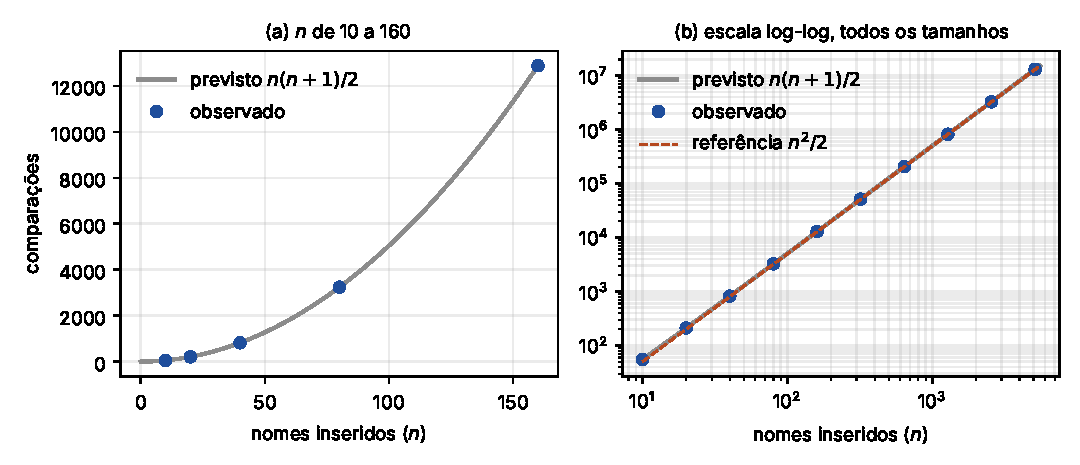
\includegraphics[width=\linewidth]{gerado/grafico.pdf}
\caption{Comparações observadas e previstas. (a) série obrigatória em escala
linear; (b) todos os tamanhos em escala log-log, com a reta de referência
$n^2/2$.}
\label{fig:grafico}
\end{figure}

\paragraph{Execução completa com redundâncias.} A Tabela~\ref{tab:completa}
resume a execução com o arquivo de origem inteiro, que contém nomes repetidos.

\begin{table}[htbp]
\centering
\begin{tabular}{lr}
\toprule
Grandeza & Valor \\
\midrule
Registros lidos da origem & 6.250 \\
Nomes inseridos ($m$) & 6.000 \\
Nomes redundantes ($d$) & 250 \\
Comparações observadas & 18.761.097 \\
$m(m+1)/2$ (custo das inserções) & 18.003.000 \\
Excesso (custo das $d$ buscas com sucesso) & 758.097 \\
Excesso médio por redundante & 3032,4 \\
\bottomrule
\end{tabular}

\caption{Execução completa sobre \texttt{bolsistas-2025.csv}.}
\label{tab:completa}
\end{table}

%--------------------------------------------------------------------------
\section{Comparação entre os resultados teóricos e empíricos}

Em todos os \totalpontos{} tamanhos medidos, de 10 a \maiorN{} nomes, o número de
comparações observado é \emph{igual} ao previsto por $C(n)=n(n+1)/2$: a diferença
é zero em cada linha das Tabelas~\ref{tab:obrigatoria} e~\ref{tab:razoes}. Os
cinco valores da série obrigatória (55, 210, 820, 3.240 e 12.880) coincidem
com o exemplo do enunciado.

Os indicadores assintóticos também concordam com a classificação $\Theta(n^2)$:
\begin{itemize}[nosep]
  \item $C(n)/n^2$ decresce e se aproxima de $1/2$ (vale \cnnMaior{} para
        $n=\maiorN$);
  \item a razão $C(n)/C(n/2)$ observada é idêntica à teórica $4(n+1)/(n+2)$ e se
        aproxima de 4 (vale \razaoMaior{} no maior $n$);
  \item o coeficiente angular da reta ajustada por mínimos quadrados a
        $\ln C(n)$ contra $\ln n$ (Figura~\ref{fig:grafico}b) é \inclinacao,
        próximo do expoente 2 (fica ligeiramente abaixo de 2 por causa da
        parcela linear $n/2$, que perde importância quando $n$ cresce).
\end{itemize}

Na execução completa (Tabela~\ref{tab:completa}) a hipótese H2 não vale, pois o
arquivo tem \cRedundantes{} nomes repetidos. As \cInseridos{} inserções custam
exatamente $m(m+1)/2=\cBase{}$ comparações, porque cada inserção percorre o
destino inteiro. O excesso de \cExcesso{} comparações corresponde às buscas dos
nomes repetidos, que terminam no ponto em que o nome é encontrado (em média
\cMedia{} comparações cada).

%--------------------------------------------------------------------------
\section{Discussão dos resultados}

\begin{enumerate}[label=\textbf{\arabic*.}]
  \item \textbf{Os dados empíricos confirmam a hipótese de complexidade?} Sim. A
        hipótese ($C(n)=n(n+1)/2$, logo $\Theta(n^2)$) previu exatamente todos
        os \totalpontos{} valores medidos, em uma faixa de $n$ que cobre mais de duas ordens de
        grandeza (10 a \maiorN).
  \item \textbf{Como se comporta a taxa de crescimento quando $n$ dobra?} A
        razão observada sobe de 3,818 (10$\to$20) a \razaoMaior{} e tende a 4,
        coerente com $C(2n)/C(n)=4-2/(n+1)$. Um algoritmo linear daria razão 2 e
        um cúbico daria 8; os dados apontam inequivocamente para o regime
        quadrático.
  \item \textbf{Há diferenças entre valores teóricos e medidos?} Não: a
        diferença é zero em todos os pontos. Isso é esperado porque o que se mede
        é uma contagem de operações, determinística, e não um tempo de
        execução, que teria ruído. Diferenças apareceriam se o modelo e o
        programa divergissem. Por exemplo: (a) se o cabeçalho não fosse comparado, o
        observado seria $n(n-1)/2$, ou seja, $n$ comparações a menos; (b) com nomes
        repetidos, a busca bem-sucedida termina antes do fim, como na execução
        completa; (c) com destino previamente preenchido, cada inserção
        começaria de um tamanho maior que 1.
  \item \textbf{Os resultados sustentam a demonstração matemática?} Sim, no
        sentido em que são consistentes com ela e verificam que o programa
        instrumentado implementa o modelo (Lema~\ref{lema:custo}). Os
        experimentos, porém, são casos particulares: quem garante a validade
        para \emph{todo} $n$ é a indução. Os dois se complementam: a prova
        garante a fórmula sob H1--H3 e as medições garantem que o
        código executa o que as hipóteses descrevem.
  \item \textbf{Qual é a evidência empírica da complexidade indicada?} Quatro
        evidências independentes: (i) igualdade exata entre observado e previsto
        em \totalpontos{} tamanhos; (ii) $C(n)/n^2\to 1/2$; (iii) razão ao
        dobrar $\to 4$; (iv) inclinação log-log \inclinacao{} $\approx 2$.
  \item \textbf{Comparação explícita dos dados com a hipótese para $C(n)$.} A
        hipótese $C(n)=n(n+1)/2$ poderia ter sido enfraquecida por razões
        distantes de 4, por inclinação log-log longe de 2 ou por diferenças
        sistemáticas observado $-$ previsto. Nenhuma ocorreu: a hipótese sai
        \emph{fortalecida}. Cabe a ressalva de que medições finitas não provam
        um resultado assintótico por si sós; aqui o resultado assintótico se
        apoia na dedução e na indução, e os dados as corroboram.
\end{enumerate}

%--------------------------------------------------------------------------
\section{Conclusão}

A função deduzida, $C(n)=\sum_{k=1}^{n}k=\dfrac{n(n+1)}{2}$, foi demonstrada por
indução matemática (caso base $C(0)=0$, hipótese $C(k)=k(k+1)/2$ e passo
$C(k+1)=C(k)+(k+1)=(k+1)(k+2)/2$). Dela decorre que o algoritmo de importação
com busca sequencial é $\Theta(n^2)$, e que dobrar o número de nomes multiplica
as comparações por $4-2/(n+1)$, tendendo a 4.

Os experimentos com o contador instrumentado deram 55, 210, 820, 3.240 e 12.880
comparações para 10, 20, 40, 80 e 160 nomes, sem nenhuma diferença em relação
ao modelo, e a série ampliada até \maiorN{} nomes manteve a igualdade exata e
aproximou $C(n)/n^2$ de $1/2$, a razão de dobra de 4 e a inclinação log-log de 2.
Assim, a hipótese de complexidade quadrática é válida à luz das evidências
empíricas, que reforçam a demonstração formal. Como observação de projeto, o
custo quadrático vem da busca sequencial, e uma estrutura indexada (por exemplo,
tabela de dispersão) reduziria o custo esperado a $O(n)$, mas sairia do escopo
do algoritmo analisado.

%--------------------------------------------------------------------------
\appendix
\section{Código-fonte (\texorpdfstring{\texttt{src/copiador.c}}{src/copiador.c})}
\lstinputlisting[basicstyle=\ttfamily\scriptsize]{../src/copiador.c}

\end{document}
